\section*{Problem 3}

Twelve jobs numbered from 1 to 12 have to be executed satisfying the following requirements:
\begin{itemize}
  \item The running time of job $i$ is $i$, for $i = 1, 2, . . . , 12$.
  \item All jobs run without interrupt.
  \item Job 3 may only start if jobs 1 and 2 have been finished.
  \item Job 5 may only start if jobs 3 and 4 have been finished.
  \item Job 7 may only start if jobs 3, 4 and 6 have been finished.
  \item Job 9 may only start if jobs 5 and 8 have been finished.
  \item Job 11 may only start if Job 10 has been finished.
  \item Job 12 may only start if jobs 9 and 11 have been finished.
  \item Jobs 5,7 en 10 require a special equipment of which only one copy is available, so no two of these jobs may run at the same time.
\end{itemize}
Find a solution of this scheduling problem for which the total running time is minimal.

\vspace{4mm}

\subsection*{Solution:}
We generalize this problem for $n$ number of jobs. First we introduce two variables $S_{i}$ and $F_{i}$ for $i = 1,2,3,...,n$.
\begin{itemize}
  \item $S_{i}$ is the starting time of Job $i$. $S_{i} \geq 0$. For example: If Job 1 starts at 0, then $S_{1} = 0$. $S_{i}$ can be any positive integer number if it is satisfied with all requirements.
  \item $F_{i}$ is the finish time of Job $i$.
\end{itemize}

Secondly, we find the clauses which have to be satisfied by all requirements of this problem.

\begin{description}

  \item[Clause 1:] We defined that the starting time of all jobs have to be greater or equal to zero. This is expressed by the formula
      \[ \bigwedge_{i=1}^n (S_{i} \geq 0).\]

  \item[Clause 2:] The running time of job $i$ is $i$, for $i = 1, 2, . . . , n$, and all jobs run without interrupt. So we have
      \[ \bigwedge_{i=1}^n (F_{i} = S_{i} + i).\]

   \item[Clause 3:] The problem specifies that there is a dependency between some jobs, for instance job 3 may only start until jobs 1 and 2 have finished. In order to generalize this and to make a compact formula, we introduce the set of dependencies $\textbf{D}_{i}$ as the set of $finish$ $times$ of the jobs that have to end before starting job $i$, for $i = 1, 2, . . . , n$. So the set of dependencies of job 3 may look like: $\textbf{D}_{3} = \{ F_{1}, F_{2} \}$. Now we can formulate the clause of dependencies between jobs as follow:
       \[ \bigwedge_{i=1}^n \bigwedge_{d \in D_{i}} (S_{i} \geq d).\]

  \item[Clause 4:] The last requirement states that there is an special equipment that can be only used by one job at a time. So the jobs that require this resource cannot work in parallel. To express this we consider the condition that if a job that requires the resource happens before another job that also needs the resource, then the later must only happen if the first job has finished.

      In order to generalize this and formulate a compact expression, we define $\textbf{P}$ as the set of all jobs that share the resource, and define the mappings $f:\textbf{P} \to \textbf{F}$ to map the jobs in $\textbf{P}$ to its respective finish time, and $s:\textbf{P} \to \textbf{S}$ to map the jobs in $\textbf{P}$ to its respective starting time, where $\textbf{F}$ and $\textbf{S}$ are the sets of all finish times and starting times.

      Using all this elements the formula that expresses this clause is the following:

      \[ \bigwedge_{p,q: \; p,q \in \textbf{P} \land p \neq q} (s(p) \leq s(q)) \Rightarrow (f(p) \leq s(q)) .\]

   \item[Clause 5:] The problem also require to find a solution of this scheduling problem for which the total running time is minimal. In order to find such scheduling, we introduce a variable $T$ to represent the allowed running time, now we have to bound the finish time of all jobs to this variable. This can be expressed with the following formula:
       \[ \bigwedge_{i=1}^n (F_{i} \leq T).\]


\end{description}


The total formula now consists of the conjunction of all these clauses.
\[ \bigwedge_{i=1}^n (S_{i} \geq 0)\;\;\wedge\]
\[ \bigwedge_{i=1}^n (F_{i} = S_{i} + i)\;\;\wedge\]
\[ \bigwedge_{i=1}^n \bigwedge_{d \in D_{i}} (S_{i} \geq d)\;\;\wedge\]
\[ \bigwedge_{p,q: \; p,q \in \textbf{P} \land p \neq q} (s(p) \leq s(q)) \Rightarrow (f(p) \leq s(q)) \;\;\wedge\]
\[ \bigwedge_{i=1}^n (F_{i} \leq T).\]


The complete formula expressed in SMT syntax choosing $n=12$, $D_{3} = \{ F_{1}, F_{2} \}$, $D_{5} = \{F_{3}, F_{4}\}$, $D_{7} = \{F_{3}, F_{4}, F_{6}\}$, $D_{9} = \{F_{5}, F_{8}\}$, $D_{11} = \{F_{10}\}$, $D_{12} = \{F_{9}, F_{11}\}$, $P = \{Job\;5, Job\;7, Job\;10\}$ and $T = 36$ is as follow:

{\footnotesize

{\tt (benchmark part1$\_$3}

{\tt :logic $QF\_UFLIA$}

{\tt :extrafuns (}

{\tt (S1 Int) (S2 Int) (S3 Int) (S4 Int)  (S5 Int)  (S6 Int)}

{\tt (S7 Int) (S8 Int) (S9 Int) (S10 Int) (S11 Int) (S12 Int)}

{\tt (F1 Int) (F2 Int) (F3 Int) (F4 Int)  (F5 Int)  (F6 Int)}

{\tt (F7 Int) (F8 Int) (F9 Int) (F10 Int) (F11 Int) (F12 Int))}

{\tt :formula (and}

{\tt (>= S1 0) (>= S2 0) (>= S3 0) (>= S4 0)  (>= S5 0)  (>= S6 0)}

{\tt (>= S7 0) (>= S8 0) (>= S9 0) (>= S10 0) (>= S11 0) (>= S12 0)}

$\cdots \cdots$

{\tt ;All jobs run without interrupt}

{\tt (= (+ S1 1) F1)}

{\tt (= (+ S2 2) F2)}

{\tt (= (+ S3 3) F3)}

$\cdots \cdots$

{\tt ;Job dependencies}

{\tt  (>= S3 F1)  (>= S3 F2)}

{\tt  (>= S5 F3)  (>= S5 F4)}

{\tt (>= S7 F3)  (>= S7 F4) (>= S7 F6)}

$\cdots \cdots$

{\tt ;Jobs 5,7 and 10 cannot execute in parallel}

{\tt (implies (<= S5 S7)   (<= F5 S7))}

{\tt (implies (<= S5 S10)  (<= F5 S10))}

{\tt (implies (<= S7 S5)   (<= F7 S5))}

$\cdots \cdots$

{\tt (<= F1 36)}

{\tt (<= F2 36)}

{\tt (<= F3 36)}

$\cdots \cdots$
}

\vspace{3mm}

Applying {\tt yices-smt -m part$1\_3$.smt} to test out a satisfiable scheduling, we got the following result:

{\footnotesize

{\tt sat}

{\tt (= S1 1)}

{\tt (= S2 0)}

{\tt (= S3 5)}

{\tt (= S4 3)}

$\cdots \cdots$

{\tt (= F5 15)}

{\tt (= F6 6)}

{\tt (= F7 32)}

{\tt (= F8 15)}

{\tt (= F9 24)}

{\tt (= F10 10)}

{\tt (= F11 24)}

{\tt (= F12 36)}
}

\vspace{3mm}

We know that this is the schedule where the total running time is minimal because we started increasing the value of $T$ from 9 and stop until the SMT is SAT. Finally, we find when $T = 35$, it is UNSAT, but when $T = 36$, it is SAT. Therefore, we conclude that the minimal running time satisfying the requirements is $36$.

The following picture illustrates such schedule:

\begin{center}
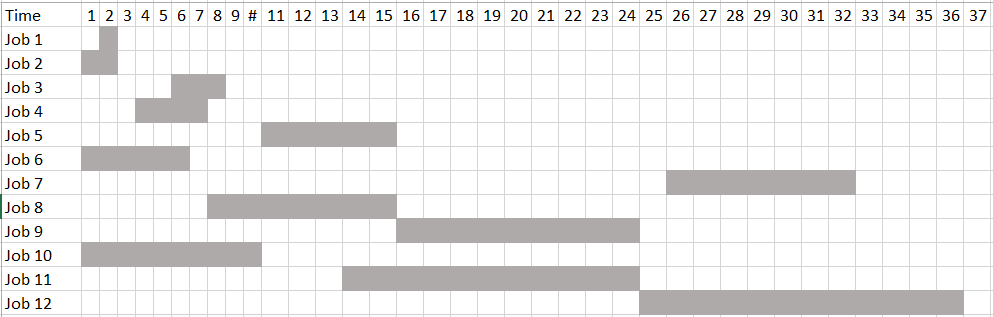
\includegraphics[width=1.0\textwidth]{Part1_3_1.png}
\end{center}

\subsection*{Remark:}

For this particular problem, the minimum running time was found testing the value of $T$ for different values until we find the minimum satisfiable. Although doing this was relatively easy because the number of jobs is small, and therefore also the minimum running time, this method of finding the minimum value by hand is not very suitable for longer number of jobs and dependencies between them. For instance, if we have $1000$ jobs with their respective dependencies, it would be very time consuming to find such value by hand. Since Yices 1.2 does not have a method for automatically find minimum values, a possible solution is to implement a script that performs the tests automatically.

\subsection*{Generalization:}

We generalized this problem for any number of jobs and dependencies between them. Since we solved this choosing the values that states the problem, it would be interesting  to know the results after changing some parameters. For instance, lets imagine that we have enough copies of the special equipment required by jobs $5$, $7$ and $10$, so they can run in parallel. For this case, the minimum running time is $33$, this is not a big improvement so maybe the money spent by buying the extra equipment does not pay off in performance. 